\section{Experiment design}\label{sec:experiment_design}
%Forsoegsopstilling, der inkludere en tegning af omraadet set oppefra med indtegning af beacons, objectern og hvor rigtige position for test person.
The implemented system's evaluation experiments are conducted in a room measuring $4.75m \times 6.5m$.
In the room, a cabinet is placed between two tables, effectively dividing the room into two smaller areas. 
In each of the smaller areas a table with six chairs is placed and on the walls are placed whiteboards.
\begin{figure}[h]
    \centering
    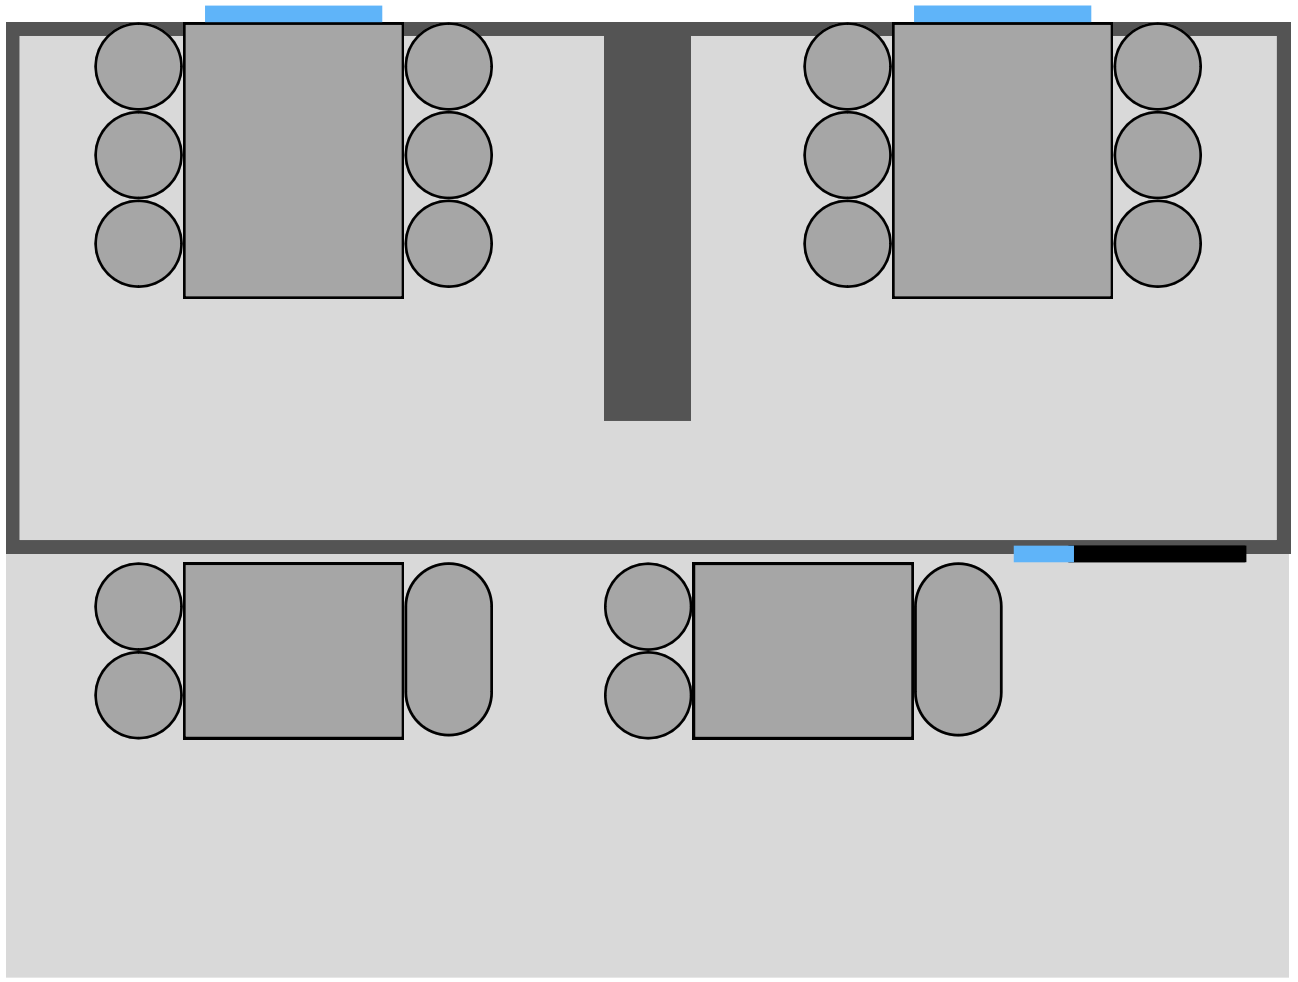
\includegraphics[scale=0.5]{images/experiment_room.png}
    \caption{A sketch of the meeting room in which the experiments were carried out.}
    \label{fig:experiment_room}
\end{figure}
On one end of each table is a large, rectangular window.
Furthermore, one table has a large TV screen placed near its window. 
Near the door of the room, an airconditioning controller and a large glass window is located. 
Next to the door is placed a glass pane, acting as a window out into the common area. 
Lighting is built into the ceiling, thus no hanging light will interfere with the broadcasted signals. 
Outside the meeting room is a common area containing two high tables.
Each of these tables has a small couch and two chairs placed next to it.
The meeting room and its surrounding area is depicted in Figure \ref{fig:experiment_room}.

Beacons are placed on top of the cabinet and in the three corners furthest away from the door. 
The beacons in the corners of the room are placed in a height of $2.5m$, while the center beacon on top of the cabinet is placed in a height of $1.5m$.   
The beacons placed near the windows are located on top of a whiteboard, while the beacon in the lower left corner of the room is held in place using painter's tape. 

\subsection{Creating a map}
To execute the first phase of the approach described in Section \ref{sec:first_phase},  we partition the previously described meeting room into a $1m \times 1m$ grid and place beacons as described using painter's tape.%Supervisor requests EXACT setup
To collect measurements for the creation of the map, a person holding a Samsung Galaxy A53 5G phone, with the application described in Section 2 installed and running, traverses systematically through the room and stops at the intersection of each grid line to collect data. 
We will refer to this person as the \textit{collector}.
With the app, it is possible to perform measurements from any number of selected beacons and append a label to the measurements.
In this experiment, the collector selects all beacons and is responsible for the correct collection and labeling of each cell.
\begin{figure}[h]
    \centering
    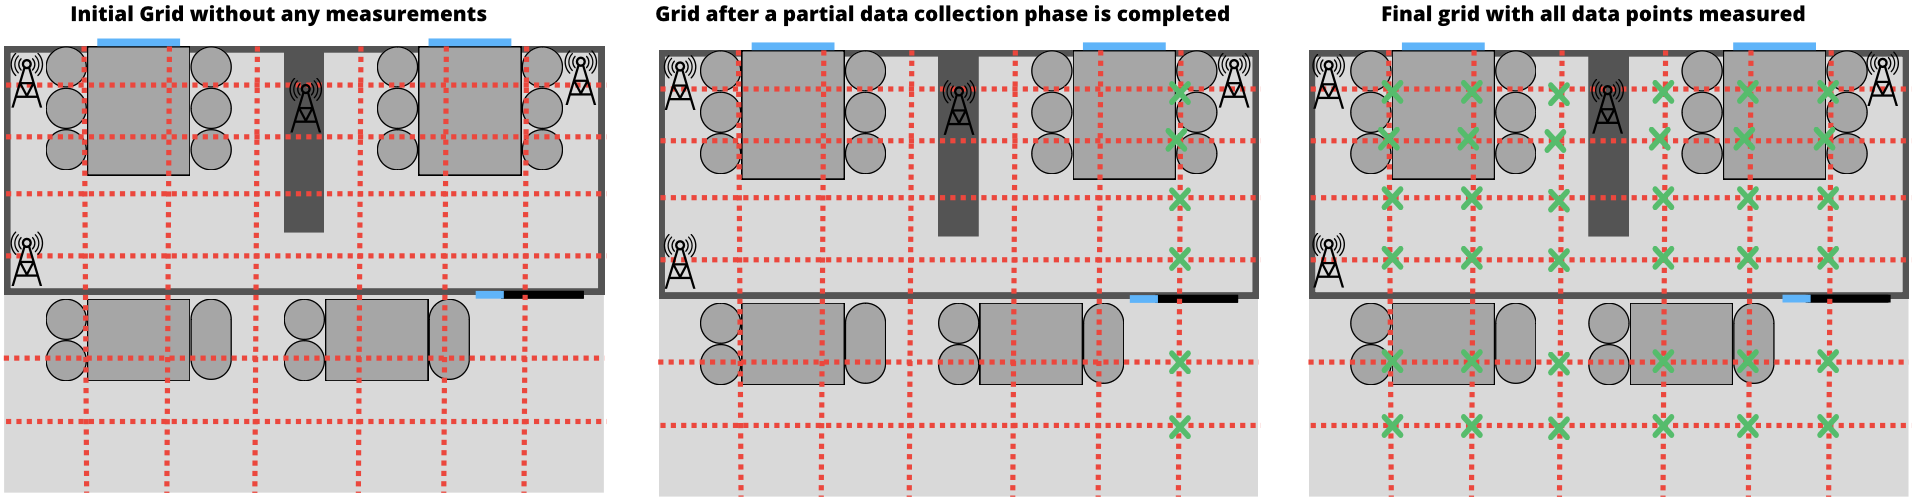
\includegraphics[width=\textwidth]{images/experiment_map_creation.png}
    \caption{A sketch of the meeting room partitioned into a grid decorated with beacon placements (red antenna) and measurement locations (circles with letters). The figure how the measurements are collected systematically in the meeting room.}
    \label{fig:experiment_map_creation}
\end{figure}
When the collector stops at the intersection of two grid-lines, they can press a button in the app, which starts measuring after a number of seconds.
The phone provides auditory feedback when it has collected enough measurements for the requirements described in Section \ref{sec:first_phase} to be fulfilled.
When the information for measurement has been computed and stored on the phone, the collector is informed auditorily and continues to the next intersection in the grid. 
During the measurement the phone is kept in roughly the same height.
Measurements are collected in a setup using 4 beacons, as depicted in Figure \ref{fig:experiment_map_creation}.
The map creation process was done during out-of-office hours to ensure that the datapoint collected to create the map was collected with a minimum of background signal noise.  

\subsection{Evaluation strategy} %This is where we examine if we can classify correctly
\begin{figure}[h]
    \centering
    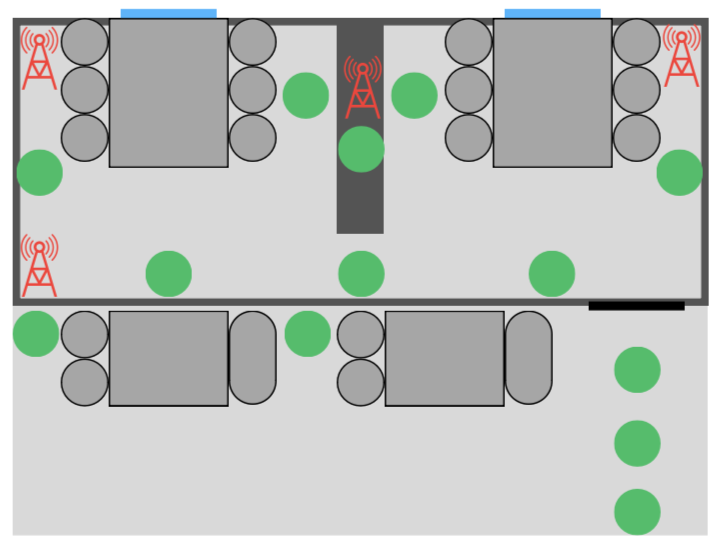
\includegraphics[scale=0.5]{images/experiment_setup.png}
    \caption{A sketch of the meeting room in which the experiments were carried out, decorated with beacon placements (red antenna) and measurement locations(green circles)}
    \label{fig:experiment_setup}
\end{figure}
In evaluating the generated map, our aim is to determine if the system can accurately distinguish whether a receiving device is situated inside or outside the room.
As described in Section \ref{sec:bluetooth_low_energy}, physical obstacles can cause fluctuations in the received signals. 
Therefore, we design the expirement such that measurements are taken in areas where some, none, and all of the beacons are blocked. 
We perform measurements in the following areas:
\begin{itemize}
    \item Along the walls inside of the meeting room, to examine border values of the map while inside the room
    \item Along both sides of the divider, to examine whether obstructions inside the room has any meaningful effect on the classification
    \item On the cabinet, next to the beacon, to examine classification of a receiver placed in the middle of the room
    \item $1$ meter, $2$ meters, and $3$ meters outside the door, to examine how far away from the meeting a receiver must be before it is classified as outside.
    \item By the tables in the common area, to ensure that we do not classify an outside area as an inside area.
\end{itemize}
For each of these areas 10 data points has been collected and classified on several devices.
Data collection points and beacon placement of the room during the experiment is shown in Figure \ref{fig:experiment_setup}. 
